\documentclass{beamer}
\setbeamertemplate{navigation symbols}{}

\mode<presentation>
{
\usetheme{Warsaw}
\usecolortheme{crane}
\setbeamercovered{transparent}
}

\usepackage[italian]{babel}
\usepackage[utf8]{inputenc}	%[latin1]
\usepackage{patlib}

% font definitions, try \usepackage{ae} instead of the following
% three lines if you don't like this look 
\usepackage{mathptmx}
\usepackage[scaled=.90]{helvet}
\usepackage{courier}
\usepackage[T1]{fontenc}
\usepackage{hyperref}
\usepackage{xfrac}
\usepackage{booktabs}% http://ctan.org/pkg/booktabs
\usepackage{ulem} %for strikeout
\usepackage{xcolor}
%\usepackage[shortlabels]{enumitem} % for letters in enumerate
%\renewcommand{\theenumi}{\Alph{enumi}}

% ----GENERALE-------------------------------------------------------------------

\title{introduzione a Bitcoin}
\subtitle{e alle criptovalute digitali}
\author{P.Bertoni}

% If you have a file called "university-logo-filename.xxx", where xxx
% is a graphic format that can be processed by latex or pdflatex,
% resp., then you can add a logo as follows: 

\pgfdeclareimage[height=0.5cm]{btclogo}{images/bitcoin.png}
%\logo{\pgfuseimage{btclogo}}

% Delete this, if you do not want the table of contents to pop up at
% the beginning of each subsection:
\AtBeginSubsection[]
{
\begin{frame}<beamer>
\frametitle{contenuto}
\tableofcontents[currentsection,currentsubsection]
\end{frame}
}

% If you wish to uncover everything in a step-wise fashion, uncomment
% the following command:
%\beamerdefaultoverlayspecification{<+->}

\begin{document}
% ----TITOLO---------------------------------------------------------------------
\begin{frame}
	\titlepage
\end{frame}
% ----SOMMARIO-------------------------------------------------------------------
\begin{frame}
	\frametitle{Tabella Contenuti}
	\tableofcontents
\end{frame}
% ----SEZIONI--------------------------------------------------------------------
\section{Introduzione}
\subsection{Problema} % %\subsection[Short First Subsection Name]{Problema}
	\begin{frame}

	\frametitle{Criptovaluta}
	\framesubtitle{specifiche sul protocollo}
	
	\textit{Problema}
	\newline implementare una {\color{blue}valuta} economica
	\begin{itemize}
	  \item sicura
	  \item basata su informatica
	  \item decentralizzata % implica distribuita; in senso lato evidenzia l'assenza di nodi master -> SAY da dove viene la fiducia?
	  \item distribuita % l'informazione (o il computo, che è più questo caso) è appunto distribuita su può nodi
	\end{itemize}

\end{frame}

	\begin{frame}
	\frametitle{Criptovaluta}
	\framesubtitle{specifiche sulle transazioni}
	
	\textit{problema} \vspace{5pt}
	\newline trasmettere {\color{blue}transazioni} di valuta tra enti
	\begin{itemize}
	  \item pubbliche
	  \item anonime $\Rightarrow$ tra \textbf{indirizzi}, non utenti
	  \item autenticate
	  \item non ripudiabili
	  \item irreversibili
	\end{itemize}
	registrate in una sorta di {\color{blue} storico} globale
	
\end{frame}
	
\begin{frame}
	\frametitle{Criptovaluta}
	\framesubtitle{idea astratta di transazione $\mathfrak{T}$}
	
	\begin{itemize}
	  \item atto tra $\orange{N}$ mittenti e $\orange{M}$ destinatari
	  \item utenti incoraggiati a usare un indirizzo unico $\forall \;\orange{\mathfrak{T}}$
	  \item $\sim$ {\color{blue}assegno}
	  \newline \textit{``in data $t$, $\{\orange{x}\}_{\,1}^N$ ha versato} tot \textit{a $\{\orange{y}\}_{\,1}^M$ che ora ne è proprietario''}
	\end{itemize}
	gestione del {\color{blue}resto}
	\begin{itemize}
		\item $\orange{y'}\in\{\orange{y}\}$ destinatari, controllato da chi
		emette $\orange{\mathfrak{T}}$
		\item deframmentare: nuova $\orange{\mathfrak{T}}$ con molteplici mittenti
	\end{itemize}
\end{frame}
	\begin{frame}

	\frametitle{Criptovaluta}
	\framesubtitle{specifiche sull'affidabilità}
	
	\textit{Problema}
	\newline progettare un algoritmo di {\color{blue}mining} per convalidare transazioni
	\begin{itemize}
	  \item \textit{trattabile} da decidere
	  \item \textit{intrattabile} da risolvere
	  \item dipendente da lista transazioni in attesa
	\end{itemize}
	motivazione a {\color{blue}partecipare} al mining
	\begin{itemize}
		\item ricompense
		\begin{itemize}
		  \item immediate
		  \item durevoli
		\end{itemize}
	  \item complessità lavoro onesto $\equiv$ complessità disonesto 
	  \item ma $\Pr[\text{successo lavoro disonesto}]\rightarrow 0$
	\end{itemize}
	
\end{frame}

	
\subsection{Caratteristiche di una criptovaluta}
	\begin{frame}
	\frametitle{Differenze con valute tradizionali}
	
\begin{table}[h]
\begin{tabular}{ll}
	%\hline
	%\multicolumn{1}{c}{} &
	%\multicolumn{1}{c}{\justfig{euro.png}{0.1}} \\
	\multicolumn{1}{c}{
\includegraphics[width = 1 cm]{images/euro.png}} &
	\multicolumn{1}{c}{
\includegraphics[width = 1 cm]{images/bitcoin.png}} 											  \\
	
	\multicolumn{2}{l}{{\color{blue}ontologia}}                                                               \\
	\multicolumn{1}{c}{esplicita: come unità fisiche} &
	\multicolumn{1}{c}{implicita: in funzione di transazione}															  \\ \hline \\
	
	\multicolumn{2}{l}{{\color{blue}fiducia nell'accettazione di moneta}}                                             \\
	\multicolumn{2}{c}{difficoltà di contraffazione}                                                                  \\ \hline \\
	
	\multicolumn{2}{l}{{\color{blue}possibilità di furto o smarrimento}}			\\
	\multicolumn{1}{c}{gettone fisico} & \multicolumn{1}{c}{chiave privata di firma digitale}                         \\ \hline \\
	\multicolumn{2}{l}{{\color{blue}fiducia nel protocollo di supporto}}                                              \\
	\multicolumn{1}{c}{ente nazionale o sovranazionale} & \multicolumn{1}{c}{modello formale di sicurezza}            \\
	\end{tabular}
\end{table}

\end{frame}
	\begin{frame}
	\frametitle{i primordi: eCash [Chaum]}
	\framesubtitle{sistema di firma digitale a \textit{conoscenza zero}}
	
	Scenario (\textit{e.g.} voto digitale)
	\begin{itemize}
	  \item sia $\orange{m}$ plaintext, $A$ il suo autore e $F$ il firmatario 
	  \item $A\neq F$
	  \item firma \textit{classica}: $\orange{S}(\orange{m},\,\orange{K_{PR}^A})$
	  \item firma \textit{{\color{blue}cieca}}: $\orange{S^B}(\orange{f}(\orange{m}),\,\orange{K_{PR}^F})$ 
	  \item $F$ non può calcolare $\orange{m}$ data $\orange{f}(\orange{m})$  
	\end{itemize}
	Algoritmo
	\begin{enumerate}
	  \item $A$ estrae \textit{nonce} $\orange{x}$
	  \item $A$ calcola e invia $\orange{\tilde{m}}=\orange{f}(\orange{m},\,\orange{x})$ messaggio \textit{blinded} 
	  \item $F$ calcola e invia $\orange{\tilde{s}}=\orange{S}(\orange{\tilde{m}},\,\orange{K_{PR}^F}) 
	  		\equiv \orange{S^B}(\orange{f}(\orange{m}),\,\orange{K_{PR}^F})$
	  \item $A$ calcola $\orange{s}=\orange{f}^{-1}(\orange{\tilde{s}}.\orange{\tilde{m}},\,\orange{x})$ firma valida
	\end{enumerate}

\end{frame}

%DIMOSTRAZIONE CON RSA
\subsection{Elementi teorici}
	\begin{frame}
	\frametitle{Curve Ellittiche}

\begin{columns}
	\begin{column}{.65\textwidth}

		\begin{itemize}
			\item curve definite su un certo $\mathbb{F}_\orange{q}$ da 
				$$y^2=x^3+\orange{a}x+\orange{b}$$
			\item non singolari, \textit{i.e.} $4a^3+27b^2\neq 0$
		\end{itemize}

		\begin{theorem}[Hasse]
			 sia $\mathbb{F}_q$ il campo di Galois di ordine $q$ 
			 \newline sia $\mathcal{E}_q=\mathcal{E}_{(a,b)}(\mathbb{F}_q)$ una sua curva ellittica 
			\vspace*{4pt}
			\begin{enumerate}
				\item $|o(\mathcal{E}_q)-(q+1)|\leq2\sqrt q$
			\end{enumerate}	
		\end{theorem} 
		$\;\;\;\Rightarrow\;\;${\color{blue}ordine} \textit{GF} governa \textit{difficoltà}

	\end{column}

	\begin{column}{.4\textwidth}
		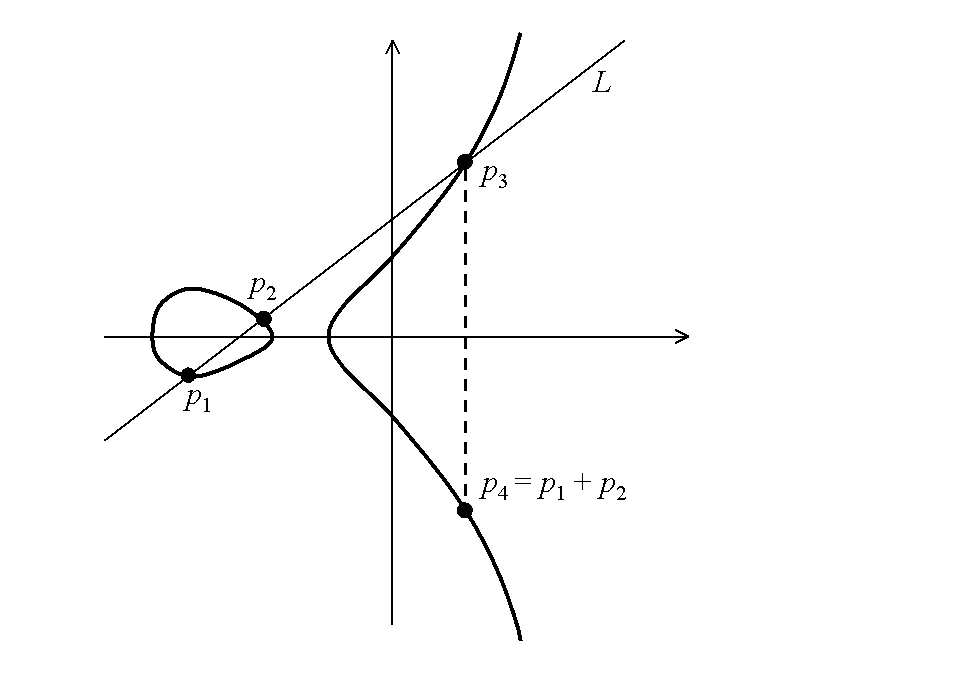
\includegraphics[height = 5 cm]{images/eca.png}
	\end{column}
\end{columns}

\end{frame}
%-------------------------------------------------------------------------
\begin{frame}
	\frametitle{Curve Ellittiche}
	\framesubtitle{legge di gruppo: definizione}
	
	$(\mathcal{E}_{(a,b)}(\mathbb{F}_q),\; \red{+})$ definisce un {\color{blue}gruppo abeliano}
	$$ \orange{R} = \orange{P}+\orange{Q} \triangleq(\orange{x_R},\,{\color{red}-}\orange{y_R}) $$
	$$x_P \neq x_Q \;: \;\;
  			\left \{ \begin{array}{lr}
	  			y_R \triangleq y_P+s(x_R-y_P) \\
				x_R \triangleq s^2-x_P-x_Q & s=\frac{y_P-y_Q}{x_P-x_Q}
			\end{array} \right. $$
			
	$$x_P = x_Q \;: \;\;
  			\left \{ \begin{array}{lcr}
 
  			y_P = -y_Q\;: & R = O \\
			 y_P = y_Q \neq 0\;: & \left\{
				  \begin{array}{lcr}
				  	y_R \triangleq y_P+s(x_R-y_P) \\
				    x_R \triangleq s^2-2x_P & s=\frac{3x_P^2+a}{2y_P}
				  \end{array}
				\right. 
			\end{array} \right. $$
 	\vspace{1pt}				
 	$$ \orange{R} = \orange{P}{\color{red}\times}\orange{n} 
 		\triangleq \orange{P}+\orange{P}+\ldots+\orange{P}\;\;\;\;\;\;\;\;\; n\in \mathbb{Z}\;\;\mathrm{volte}$$
	
\end{frame}
%-------------------------------------------------------------------------
\begin{frame}
\frametitle{Curve Ellittiche}
	\framesubtitle{legge di gruppo: casistica}
	
	\begin{figure}[H]
	 	\begin{center}
			 \begin{tabular}{c @{\hspace{1em}} c}
				 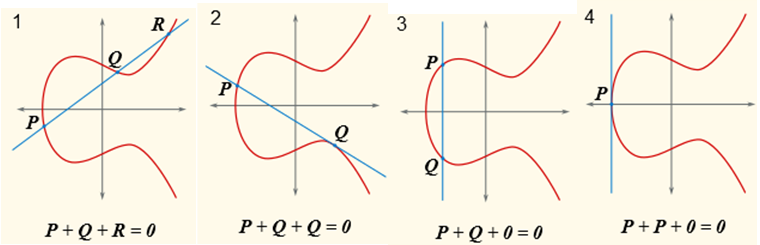
\includegraphics[width = 11 cm]{images/ecalgebrarow.png}
			 \end{tabular}
		 \end{center}
 	\end{figure}
	
\end{frame}	
%-------------------------------------------------------------------------
\begin{frame}
	\frametitle{Curve Ellittiche}
	\framesubtitle{problema matematico}
	
	%$(\mathcal{E}_{(a,b)}(\mathbb{F}_q),\,+)$ è un gruppo abeliano
% 	\begin{itemize}
% 		\item chiusura
% 		\item associatività
% 		\item identità %SAY come visto prima
% 		\item invertibilità %SAY come visto prima
% 		\item commutatività
% 	\end{itemize}  
	
	trovare un segreto ${\color{red}d}\in[1,\,n-1]$, dati
	\begin{itemize}
	  \item $\orange{\mathcal{E}}=\mathcal{E}_{(a,b)}(\mathbb{F}_q)$
	  \item $\orange{G}\in \mathcal{E}:\;\;\;\;\;\;\tiny{<}\,G\,\tiny{>}=\mathcal{E}$
	  \item $\orange{n}=o(G):\;G\times n= O=P_\infty$, $\;\;	\;n\;$ primo
	  \item $\orange{P}\in \mathcal{E}$
	  \item $\orange{Q}=P\times d$
	\end{itemize}
\end{frame}
	\begin{frame}
	\frametitle{Funzioni di Hash One Way}

	\begin{itemize}
		\item $\orange{h}:\orange{\mathbb{Z}}\rightarrow \orange{\mathbb{Z}_n}$ non iniettiva

		\item resistenza a
		\begin{itemize}
			\item preimmagine $\rightarrow$ ricerca \textit{bruta} è $O(\orange{2^n})$
			\item collisioni deboli $\rightarrow$ \;\;\;\;\; ''\;\;\;\;\; ''\;\;\;\;\; ''
			\item collisioni forti $\rightarrow$ \textit{birthday}: ricerca \textit{bruta} è $O(\orange{2^{\sfrac{n}{2}}}) \ll O(2^n)$
		\end{itemize}
		
		\item usate soprattutto per
		\begin{itemize}
		  \item autenticazione
		  \item integrità
		\end{itemize}
		\item spesso firmato il {\color{blue}digest} $\orange{h}(\orange{m})$ anzichè $\orange{m}$
	\end{itemize}

\end{frame}
	\begin{frame}
	\frametitle{Alberi di Merkle}
	
\begin{columns}
 \begin{column}{.72\textwidth}

		usati in protezione {\color{blue}integrità transazioni} %�
		\begin{itemize}
			\item foglia $\leftrightarrow\; \mathfrak{T}$
			\item $\neg$ foglia $\leftrightarrow$ hash dei due figli
			\vspace{5pt}
			\item decidere se una foglia $\in$ 
			\begin{itemize}
				\item lista: $O(\orange{N})$
				\item albero: $O(\orange{\log_2 N}) \ll O(N)$
				
			\end{itemize}
			\vspace{5pt}
			\item Bitcoin: $\;\mathrm{hash}(\orange{n})=SHA_{256}(SHA_{256}(\orange{\mathcal{L}_n}|\orange{\mathcal{R}_n}))$
		\end{itemize}

	\end{column}

	\begin{column}{.4\textwidth}
		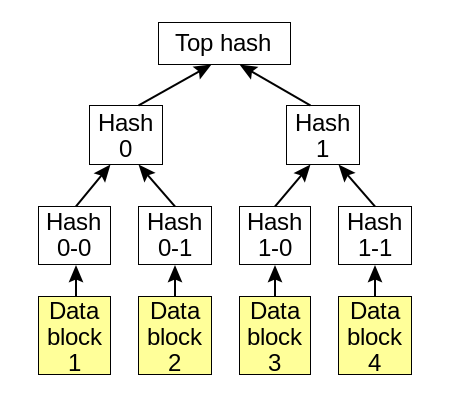
\includegraphics[height = 4 cm]{images/merkle.png}
	\end{column}
\end{columns}

\end{frame}
% -------------------------------------------------------------------------
\section{Protocollo}
\subsection{Strutture dati}
	\begin{frame}
	\frametitle{Transazione $\mathfrak{T}$}
	\framesubtitle{struttura dati}
	
	\begin{table}
	  \centering
	  \begin{tabular}{l}
	  	%sia $\orange{\mathfrak{T}_{-1}}$ \textit{precedente} a $\orange{\mathfrak{T}}$ \\
	    $\bullet\;\orange{\mathfrak{T}^{ID}}=\text{hash}(\mathfrak{\orange{T}})$\\
	    $\bullet\;$ timestamp $\orange{t}$ \\ \\
	    \begin{tabular}{l|l}
			$\bullet\;\forall i$ indirizzo di {\color{blue}input}  $\orange{\mathfrak{I}_i^{in}}$ & 
			$\bullet\;\forall j$ indirizzo di {\color{blue}output} $\orange{\mathfrak{I}_j^{out}}$ \\
			\tabitem \sout{somma trasferita $\bitcoinA_i^{in}$} & \tabitem somma ricevuta $\orange{\bitcoinA_j^{out}}$ \\
			\tabitem chiave $\orange{K^{PB}_{i,\,in}}$ & \tabitem $\text{hash}(\orange{K^{PB}_{j,\,out}})$ \\
			\tabitem indice $\orange{p}: \mathfrak{I}_i^{in}=[\mathfrak{I}_p^{out}]_{\orange{\mathfrak{T}_{-1}}}$ \\
			\tabitem $\orange{\mathfrak{T}^{ID}_{-1}}=\text{hash}(\orange{\mathfrak{T}_{-1}})$ \\
			\tabitem firma
			$\orange{\mathfrak{T}^{S_i}}=E(\orange{\tilde{\mathfrak{T}}_i},\,\orange{K^{PR}_{i,\,in}})$
		\end{tabular}		
	  \end{tabular}
	\end{table}

\end{frame}

\begin{frame}
	\frametitle{Transazione $\mathfrak{T}$}
	\framesubtitle{collegamento tra transazioni}

	\begin{figure}[H]
		\begin{center}
			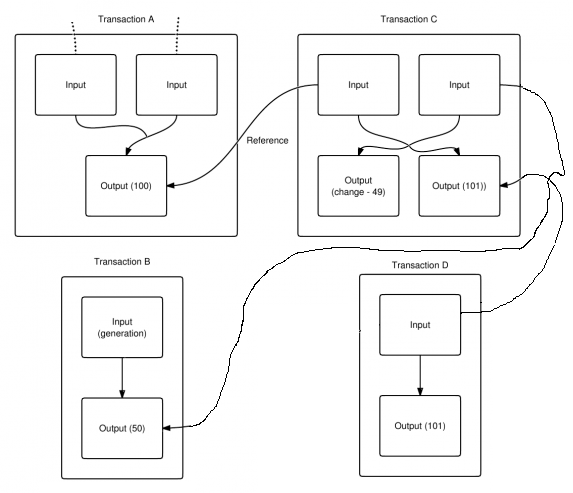
\includegraphics[height = 7 cm]{images/ref.png}	
		\end{center}
	\end{figure}

\end{frame}
	\begin{frame}
	\frametitle{Blocco $\mathfrak{B}$}
	\framesubtitle{struttura dati} 
	
	\begin{table}
	  \centering
	  \begin{tabular}{ll}
	   	{\color{blue}Header} & {\color{blue}Payload} \\
			\tabitem hash del blocco $\mathfrak{B}_{i-1}$ & \tabitem lista transazioni $\{\mathfrak{T}\}_\mathfrak{B}$ \\
			\tabitem MerkleTree di $\{\mathfrak{T}\}_\mathfrak{B}$ \\
			\tabitem timestamp corrente \\
			\tabitem target $z$ (vedi dopo)\\
			\tabitem nonce $x$ \\
			\tabitem titolare $\mathfrak{T}$ di \textit{coinbase} (vedi dopo)
	  \end{tabular}
	\end{table}
	
	\begin{itemize}
		\item durante \textit{mining} di $\mathfrak{B}$, campi continuamente modificati
		\item $\mathfrak{B}$ descrive la propria \textit{proof of work}
		\begin{itemize}
			\item \textit{input}: header di $\mathfrak{B}$ 
			\item \textit{funzione hash}: $\text{SHA}_{256}(\text{SHA}_{256}(\cdot))$
		\end{itemize} 
	\end{itemize}

\end{frame}
	\begin{frame}
	\frametitle{Transazioni $\rightarrow$ Blocchi} 
	\framesubtitle{generazione nuova transazione}
	
	\begin{enumerate}
		\item broadcastata nella rete tramite protocollo \textit{flooding}
		\item ogni miner \textbf{può} includerla nel suo \textit{pool}
		\item \textit{invalida} fino a risoluzione del $\mathfrak{B}$ ove viene inserita
		\item a quel punto chi l'ha ancora in pool la rimuove
	\end{enumerate}

	\begin{figure}[H]
		\begin{center}
			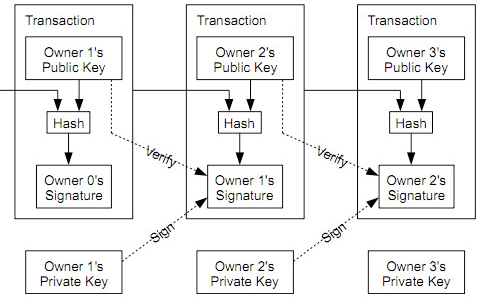
\includegraphics[height = 4.5 cm]{images/chain_transactions.png}	
		\end{center}
	\end{figure}
\end{frame}
	\begin{frame}
	\frametitle{Blocchi $\rightarrow$ Blockchain} 
	\framesubtitle{generazione catena di blocchi}
	
		\begin{itemize}
			\item hash dei blocchi precedenti \vspace{1pt} $\sim$ \vspace{1pt} puntatori di una lista
			\item a ritroso si giunge al $\mathfrak{B}$ di \textit{genesi}
		\end{itemize}
		
	 	\begin{figure}[H]
			\begin{center}
				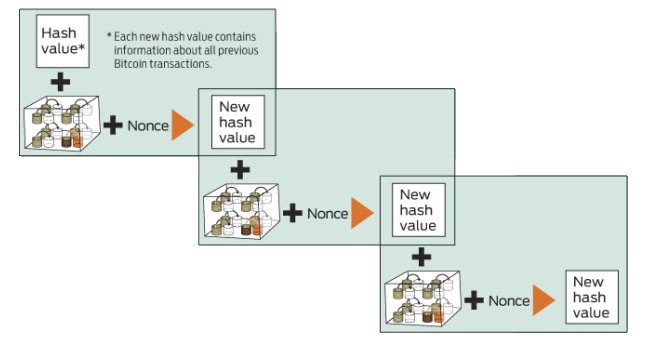
\includegraphics[height = 4.5 cm]{images/blockchain.png}	
			\end{center}
		\end{figure}

\end{frame}
	%\input{frames/motivazione_mining} %deve essere invitante lavorare per la rete, non contro essa
	\begin{frame}
	\frametitle{Motivazione all'utilizzo}
		\framesubtitle{transazioni Coinbase $\mathfrak{C}$}
		
		\begin{itemize}
			\item $\forall \mathfrak{B},\; \exists!\:\mathfrak{C}$
			\item inputs: $\emptyset$
			\item outputs: miners che han risolto $\mathfrak{B}$ 
			\item ricompensa 
			\begin{itemize}
			  	\item 50 \bitcoinA\; iniziali [2009]
				\item dimezzata ogni 210K blocchi risolti %SAY formalmente è una funzione dell'altezza blockchain
				\item nulla dopo 6.93M blocchi $\;\;\;[$previsto 2140 A.D.$]$
				\newline $\;\;\;\Rightarrow \;\; \sum_{i=0}^{6.93M-1}{\frac{50}{2^{\lfloor\sfrac{i}{210K}\rfloor}}}=21M$ \bitcoinA 	
			\end{itemize}
			\item inflazione 
			\begin{itemize}
				\item dettata solo da mining %SAY poco controllabile
				\item limitata %SAY somma massima in circolazione non modificabile
			\end{itemize}
		\end{itemize}
		
\end{frame}

% A special kind of transaction, called a coinbase transaction, has no inputs. 
% It is created by miners, and there is one coinbase transaction per block. 
% 
% Because each block comes with a reward of newly created Bitcoins (e.g. 50 BTC for the first 210,000 blocks), 
% the first transaction of a block is, with few exceptions, the transaction that grants those coins to their recipient (the miner). 
% In addition to the newly created Bitcoins, the coinbase transaction is also used for assigning the recipient of any transaction fees 
% that were paid within the other transactions being included in the same block. 
% 
% The coinbase transaction can assign the entire reward to a single Bitcoin address, 
% or split it in portions among multiple addresses, just like any other transaction. 
% 
% Coinbase transactions always contain outputs totaling 
% the sum of the block reward plus all transaction fees collected from the other transactions in the same block.
% The coinbase transaction in block zero cannot be spent. 
% This is due to a quirk of the reference client implementation that would open the potential for a block chain fork 
% if some nodes accepted the spend and others did not[1].
% capito: significa che sicuramente nel primo blocco han circolato, ma dal secondo è come se si fossero congelati e divenuti inutilizzabili

	\begin{frame}
	\frametitle{Motivazione all'utilizzo}
		\framesubtitle{fees $\mathfrak{F}$ sulle transazioni}
		
		$\forall$ transazione $\orange{\mathfrak{T}}$
		\begin{itemize}
			\item $\orange{\mathfrak{F}} = \sum_i^N \orange{\mathbb{B}_i^{in}} - \sum_i^M \orange{\mathbb{B}_i^{out}} \geq 0$
			\item spetta a miners che risolvono $\mathfrak{B}\ni\mathfrak{T}$
			\item $ \left \{
					  \begin{array}{lcr}
					    \text{\textbf{mai} obbligatoria, ma\ldots}\\ %SAY d'altronde
					    \text{miners \textbf{mai} obbligati ad aggiungere}\:\mathfrak{T}\:\text{a proprio pool di lavoro}  %SAY l'importante è risolvere il blocco, per loro un problema vale l'altro
					  \end{array}
					\right. $  
		\end{itemize}
		\vspace{5pt}
		$  \;\;\; \Rightarrow$ fees {\color{blue}incentivi} per
		\begin{itemize}
			\item velocizzare validazione di $\mathfrak{T}$
			\item \textit{mining} costante nonostante decrescita \textit{coinbase rewards}
		\end{itemize}

\end{frame}
\subsection{Primitive criptografiche} %forse, ma non credo, vanno in testa alla sezione
	% DOMANDE TEORICHE:
% 1 - DIMOSTRARE CORRETTEZZA FIRMA
% 2 - DIMOSTRARE ATTACCO CON STESSO K

\begin{frame}
	\frametitle{ECDSA}
	\framesubtitle{inizializzazione}

{\color{blue}Alice}: scelta dei parametri \textbf{pubblici}
	\begin{enumerate}
	  \item $\orange{q}=2^\orange{m}$
	  \item $(\orange{a},\,\orange{b}):\;4a^3+27b^2\neq 0$
	  \item ${\color{orange}G}=(x_G,\,y_G) \in \mathcal{E}_{(a,b)}(\mathbb{F}_q)$ 
	  \item ${\color{orange}n}=o(G)$
	\end{enumerate}
{\color{blue}Alice}: generazione coppia chiavi
	\begin{enumerate}
	  \item $K^{PR}\triangleq {\color{orange}d_A}\leftarrow \mathrm{rand} \in[1,\,n-1]$
	  \item $K^{PB}\triangleq {\color{orange}Q_A} \leftarrow {\color{orange}n}\times {\color{orange}d_A}$
	\end{enumerate}
{\color{blue}Bob}: verifica validità di $Q_A$ ricevuta
	\begin{enumerate}
	  \item $Q_A\neq O$
	  \item $Q_A\in \mathcal{E}$
	  \item $Q_A\times n=O$
	\end{enumerate}
\end{frame}
% -----------------------------------------------------------------------------
\begin{frame}
\frametitle{ECDSA}
\framesubtitle{firma digitale}

	{\color{blue}Alice}: firma del messaggio ${\color{orange}m}$ 
	\begin{enumerate}
	  \item $e \leftarrow \mathrm{hash}(m)$  %se scommento sotto, diventa e
	  % SOLO SU WIKI LETTA \item $z \leftarrow \lceil\log_2 n\rceil$ bit più a sinistra di $e$
	  \item $k \leftarrow \mathrm{rand} \in [1,n] \subset \mathbb{N}$
	  \item $(x_1,y_1) \leftarrow k \times G$
	  \item $r \leftarrow x_1\mod n$ %\\ $\;\;\;\;$ 
	  \item \textbf{if} $r=0$ \textbf{goto} 2
	  \item $s \leftarrow k^{-1}(e+rd) \mod n$ %\\ $\;\;\;\;$ 
	  \item \textbf{if} $s=0$ \textbf{goto} 2
	  \item \textbf{return} $({\color{orange}r},\,{\color{orange}s})$
	\end{enumerate}
\end{frame}
% -----------------------------------------------------------------------------
\begin{frame}
\frametitle{ECDSA}
\framesubtitle{verifica firma}	

	{\color{blue}Bob}: verifica firma $(r,s)$ di $m$
	\begin{enumerate}
	  \item $(r,\,s)\in [1,\,n-1]\times[1,\,n-1]$
	  \item $e \leftarrow \mathrm{hash}(m)$  %se scommento sotto, diventa e
	 	%SOLO SU WIKI LETTA \item $z \leftarrow \lceil\log_2 n\rceil$ bit più a sinistra di $e$
	  \item $w=s^{-1} \mod n$ 
	  \item $(u_1,\,u_2) \leftarrow (ew\mod n,\;rw \mod n)$
	  \item $(x_1,\,y_1) \leftarrow u_1 \times G + u_2 \times Q$
	  \item \textbf{ok} $\Leftrightarrow \orange{r} \equiv \orange{x_1} \mod \orange{n}$
	\end{enumerate}
\end{frame}
	\begin{frame}
	\frametitle{SHA-256}
	\framesubtitle{Secure Hash Algoritm 256 bit}
	
	\begin{itemize}	 
			\item $\sfrac{256}{2}=128$ bit di sicurezza $\Rightarrow$ collisioni non ancora trovate 
			\item $\mathrm{len}(m)\leq 2^{64}-1$
	\end{itemize}

	\begin{columns}
	 \begin{column}{.65\textwidth}
		\begin{enumerate}	 
		  	\item padding: $\mathrm{len}(m|0\dots)\equiv448\mod512$
			\item padding con 64 bit di $\mathrm{len}(m)$  
			\item $N$ blocchi da 512 bit: $\; B^{(1)},\,\dots B^{(N)} $
			\item $$ H^{(i)} \triangleq H^{(i-1)}+C_{B^{(i)}}(H^{(i-1)})$$
			\item ritorna $d=H^{(N)}$
		\end{enumerate}
	 \end{column}
	
	 \begin{column}{.55\textwidth}
	 	\begin{figure}
		 	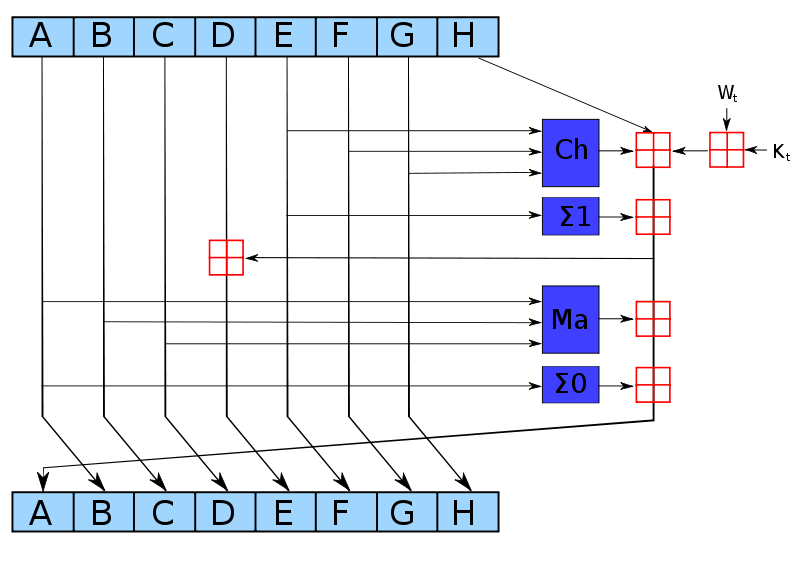
\includegraphics[height = 4 cm]{images/sha2.png}
		 	\caption{funzione di compressione $C$}
	 	\end{figure}
	 \end{column}
	\end{columns}

\end{frame}
\subsection{Modello formale di sicurezza}
	\begin{frame}
	\frametitle{Firma digitale}
	
	\begin{itemize}
		\item $|K_{ECC}|=256$ bit $\simeq |K_{RSA}|=3072 $ bit
		\item $\orange{q}\simeq 10^{\orange{77}},\;\;\orange{n}\simeq 10^{\orange{69}},
				\;\;\mathcal{E}:y^2=x^3+\orange{0}x+\orange{7}$
	\end{itemize}
	
	\begin{itemize}
	  	\item {\color{blue} meet in the middle} [Shank]: $\;\;\;\;\Omega(\sqrt{\orange{q}})$
		\item nonce $\orange{k}$ è confidenziale: $\;\;\;\;d=\red{r}^{-1}(k\red{s}-\red{e})$
		\item {\color{blue} replay attack:} nonce deve tale
		\begin{enumerate}%[label=\Alph*]
		  	\item[a)] $r_1=r_2=r$
			\item[b)] $\red{s_1}\equiv k^{-1}(\red{e_1}+d\red{r})\mod \red{n}$ 
					  $,\;\;\;\; \red{s_2}\equiv k^{-1}(\red{e_2}+d\red{r})\mod \red{n}$
			\item[c)] $k(s_1-s_2)\equiv(e_1-e_2)\mod n$
			\item[d)] $m_1\neq m_2 \Rightarrow (s_1-s_2)\neq 0\Rightarrow
			k\equiv(s_1-s_2)^{-1}(e_1-e_2)\mod n$
		\end{enumerate}
	\end{itemize} 

\end{frame}

	\begin{frame}
	\frametitle{Proof of Work}
	\framesubtitle{metodo Hashcash}
	
	\begin{itemize}
	  \item nato per contrastare spam, DoS: serve un'operazione onerosa
	  \item \textit{facile} verificare che il messaggio è soluzione di problema \textit{difficile}
	  \item {\color{blue}brute force} unica tecnica risolutiva 
	  \item Problema: dati $h:\mathbb{Z}\rightarrow\mathbb{Z}_n,\,m,\,z \leq n$, trovare nonce $x:$
	  		%$$d=h(m|x) < T_z = \sum_{i=1}^{n-z}{2^i}$$ 
	  		$$d=\orange{h}(\orange{m}|\orange{x}) < T_z = \orange{2^{n-z+1}}$$
	   		\textit{i.e.} \textbf{digest ha $z$ zeri non significativi} (parametro {\color{blue}target})
	  		$$\Pr[d<T_z|Z=z]=\frac{1}{2^z} \Rightarrow \orange{O(2^z)}$$ %SAY dimensione media esponenziale della ricerca
	  \item problema risolto $\Leftrightarrow$ blocco $\mathfrak{B}$ risolto $\Leftrightarrow \{\mathfrak{T}\}_\mathfrak{B}$ convalidate  
	  \end{itemize}
\end{frame}
% ----------------------------------------------------------------------------------------------------------------------------
\begin{frame}
	\frametitle{Proof of Work}
	\framesubtitle{exempli gratia: $z=15$}	
	 
	$$ \mathrm{hash}(\mathrm{``hello\,world''}|001)=              9002381300129484192947128  $$
	$$ \vdots \;\;\;\;\;\;\;\;\;\;\;\;\;\;\;\;\;\;\;\;\;\;\;\;\;\;\;\;\;\; \vdots$$
	$$ \mathrm{hash}(\mathrm{``hello\,world''}|034)={\color{red}0000}834716283947104512438 $$
	$$ \vdots \;\;\;\;\;\;\;\;\;\;\;\;\;\;\;\;\;\;\;\;\;\;\;\;\;\;\;\;\;\; \vdots$$
	$$ \mathrm{hash}(\mathrm{``hello\,world''}|415)={\color{green}00000000000000000000}83201 $$
	\newline
	{\color{blue}n.b.} \textit{gambler's fallacy}
	$$\forall t_1,t_2 \;\;\; \Pr(Z=z, T=t_1)=\Pr(Z=z, T=t_2)$$

\end{frame}
% ----------------------------------------------------------------------------------------------------------------------------
\begin{frame}
	\frametitle{Proof of Work}
	\framesubtitle{adattamento target}
	
	\begin{itemize}
		\item target $z_i$ ricalcolato ogni 2016 blocchi risolti $\sim$ 2 settimane
		\item $\Delta_i \leftarrow t_{i} - t_{i-1}$
		\item $\Delta_i \leftarrow \mathrm{clip}(\Delta_i,\,0.5,\,8)$
		\item $z_{i+1} \leftarrow z_i\;\frac{\Delta_i}{2}$
		\item $z \propto \Delta \Rightarrow$ {\color{blue}soluzioni veloci} abbassano target 
			\newline $\;\;\;\;\text{\textit{i.e.}}$ generazione {\color{blue}problemi più difficili}, vv.
		\item blocco risolto mediamente ogni 10 minuti
	\end{itemize}
\end{frame}
% ----------------------------------------------------------------------------------------------------------------------------
\begin{frame}
	\frametitle{Proof of Work}
	\framesubtitle{sicurezza di SHA256}
	
	in teoria\ldots
	\begin{itemize}
		\item {\color{blue}preimage attack} attack: $O(2^{256})$
		\item {\color{blue}birthday attack}: $O(2^{\sfrac{256}{2}})$
	\end{itemize}
	
	\ldots in pratica
	
	\begin{table}
	    \begin{tabular}{l|l|l|l}
		    \textit{Metodo}             & \textit{Attacco}           & \textit{Iterazioni} & \textit{Complessità} \\ \hline
		    deterministico     & collisione        & 24         & $2^{28.5}$ \\  %TODO approfondire
		    meet in the middle & preimmagine       & 42         & $2^{248.4}$ \\ %TODO approfondire
		    differenziale      & pseudo collisione & 46         & $2^{178}$ \\
		    biclique           & preimmagine       & 45         & $2^{255.5}$ \\
	    \end{tabular}
	\end{table}
\end{frame}
% ----------------------------------------------------------------------------------------------------------------------------
\begin{frame}
	\frametitle{Proof of Work}
	\framesubtitle{prevenzione double spending}
	
	per spendere due volte la stessa $\mathfrak{T}$ occorre
	\begin{itemize}
		\item modificarne gli output $\Rightarrow \mathfrak{T}$ stessa $\Rightarrow \mathfrak{B}$ di appartenenza
		\item ricalcolare nonce $x$ per $\mathfrak{B}$ modificato
		\item modifica $\mathfrak{B} \Rightarrow $ modifica di $N$ blocchi successivi
		\item ricalcolare $N$ nonces $\Rightarrow$ risolvere $N$ problemi esponenziali
	\end{itemize}
	
	\vspace{1pt}
	
	\begin{figure}[H]
	 	\begin{center}
			 \begin{tabular}{c @{\hspace{1em}} c}
				 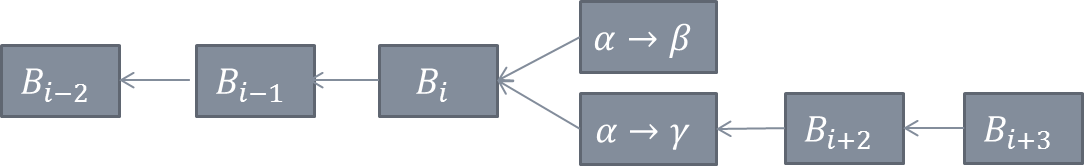
\includegraphics[width= 11cm]{images/dspending_ppt.png}
			 \end{tabular}
		 \end{center}
 	\end{figure}
 	{\color{blue}forking}
 	\begin{itemize}
 	  \item risolto imponendo aggiunta a ramo più lungo
 	  \item sotto ipotesi \textit{web of trust} sopravviverà il ramo corretto
 	\end{itemize}	
\end{frame}
	\begin{frame}
	\frametitle{Web of trust}
	
	dato un pool di miners $\mathfrak{M}$ con capacità di calcolo $\mathcal{C}_\mathfrak{M} \;\;[\sfrac{\mathrm{GH}}{\mathrm{s}}] $ \newline

	$\Pr[\mathfrak{M} \mathrm{\;risolva\;blocco}] \propto \frac{\mathcal{C}_\mathfrak{M}}{\mathcal{C}_{\Omega}} $\newline

	$\Rightarrow$ Bitcoin funziona solo se $\mathcal{C}_{\Theta} \geq 50\%\;\mathcal{C}_{\Omega} $ \newline

	se $\exists\;\mathfrak{M}_{\overline{\Theta}}$ pool disonesto: $\mathcal{C}_{\mathfrak{M}_{\overline{\Theta}}} \geq 50\%\;\mathcal{C}_{\Omega} $ \newline

	$\Rightarrow$ catena più lunga comanderebbe $\Rightarrow$ crollo fiducia $\Rightarrow$ crollo valore \newline
	\begin{itemize}
		\item no motivazione di lucro diretto
		\item ma no difesa contro nemici abbastanza potenti e motivati
	\end{itemize}
	
\end{frame}

% -------------------------------------------------------------------------
\section{Attacchi tipici}
\subsection{Forgiatura}
	\begin{frame}
	\frametitle{attacco alla firma digitale}
	
	unico modo per forgiare \bitcoinA: usare quelli di qualcuno
	\begin{itemize}
	  \item il problema di forgiare dal nulla \textbf{non ha senso}
	  \item  occorre appropriarsi di $K_{PR}\;\Rightarrow$ rompere ECDSA %SAY la cui sicurezza è già stata analizzata
	\end{itemize}
	se {\color{blue}quantum computers} implementati 
	  \begin{itemize}
	    \item rottura ECDSA può diventare \textit{facile}
	    \item inversione $\mathrm{SHA}_{256}$ resta \textit{difficile}
	  	\item indirizzi $\;\orange{\mathfrak{I}} = \mathrm{SHA}_{256}(\mathrm{SHA}_{256}(\orange{K_{PB}}))$
		\begin{itemize}
		    \item ottenere $K_{PB}$ dal solo $\mathfrak{I}$ è \textit{difficile}
		    \item ma se è nota il sistema è rotto %SAY possibilissimo
		\end{itemize}
	  \end{itemize}
\end{frame}
	\begin{frame}
\frametitle{caso di studio: Mt.GoX [2014]}
\framesubtitle{prima del crollo}
	
	{\color{blue} exchange}
	\begin{itemize}
	  \item web service di scambio valute \textit{fiat} con \bitcoinA
	  \item 2011: compromissione account interno al perimetro $\Rightarrow$ furto \bitcoinA
	  \item 2013: Blockchain fork in rami con regole diverse 
	  \newline $\;\;\;\;\Rightarrow$ MtGox sospende transazioni
	\end{itemize}
	
	{\color{blue} malleabilità}
	\begin{itemize}
		\item $\mathfrak{T}^{ID}\triangleq h(\mathfrak{T}),\;\;\;S\in\mathfrak{T}$
	 	\item codice \textit{MtGox} non controlla la validità del formato di $S$
	 	\item problema $\in$ implementazione, $\mathbf{\notin}$ protocollo \bitcoinA
	 	\item $\exists$ altri sistemi migliori per proprio storico $\Rightarrow$ immunità
	\end{itemize}

\end{frame}

\begin{frame}
\frametitle{caso di studio: Mt.GoX [2014]}
\framesubtitle{il crollo: attacco delle transazioni \textit{mutanti}}

	{\color{blue} frode} di \textit{Eve} ai danni di \textit{MtGox}
 	\begin{enumerate}
 	  	\item $M$ invia $\orange{\mathfrak{T}}$ a $E$ dopo legittima richiesta prelievo
	 	\item $E$ ritocca $\orange{S}(\orange{\mathfrak{T}})$ prima della sua conferma
	 	\item ora $\exists\,\orange{\tilde{\mathfrak{T}}}\equiv\orange{\mathfrak{T}},\;$ 
	 			ma $\orange{h}(\orange{\tilde{\mathfrak{T}}})\neq \orange{h}(\orange{\mathfrak{T}}) \Rightarrow 
	 			\orange{\tilde{\mathfrak{T}}^{ID}}\neq\orange{\mathfrak{T}^{ID}}$ 
	 	\item $\orange{\tilde{\mathfrak{T}}}$ diffusa da $E$ e confermata prima di $\orange{\mathfrak{T}}$
	 	\item $\orange{\mathfrak{T}}$ non confermata perchè $\orange{\tilde{\mathfrak{T}}}$ invalido
	 	\item $E$ manda un complain a $M$ per $\orange{\mathfrak{T}}$ non ricevuta
	 	\item $M$ controlla il suo storico: $\orange{\mathfrak{T}}$ non è stata accettata
	 	\item $M$ costretto a inviare $\orange{\mathfrak{T}^\prime}$ come rimborso
 	\end{enumerate}

	{\color{blue} DDoS}
	\begin{enumerate}
	  	\item $M$ riceve tante transazioni mutanti
	  	\item grande sovraccarico, persino se c'è resistenza a frode
	  	\item latenza nelle risposte $\Rightarrow$ incertezza $\Rightarrow$ speculazione
	\end{enumerate}

\end{frame}

% questa è L'ALTRA VERSIONE.
% NON tutte le cose utilizzate nell'hash sono anche firmate
% è possibile modificare una T in modo che l'hash ovviamente cambi, 
% ma la firma resti valida!!!!
% non è quindi safe accettare una catena di transazioni NON confermate

%This would have left Mt. Gox's ledgers increasingly out of balance with the public blockchain record.

% More importantly, the integrity of the Bitcoin network itself was never under threat. 
% TXIDs are used only for tracking bitcoin transfers by second-layer software, and their malleability has no impact on the actual transfer of bitcoin. 
% This is why the issue has not been a high priority for repair since it came to developers' attention in 2011.
% "The core software itself, we made zero changes to it, and we plan to make zero changes to it," says Garzik. 
%While the price of bitcoin staggered immediately following Mt. Gox's announcement, it rebounded as the limited nature of the problem became clear, 
%and has remained stable since -- though still at about 50\% of its early-December high.

% MENEZES!!!!!!
% A public-key encryption scheme is said to be non-malleable if given a ciphertext, 
% it is computationally infeasible to generate a different ciphertext such that the respective plaintexts are related in a known manner.
% If a public-key encryption scheme is non-malleable, it is also semantically secure.



\subsection{Anonimità}
	\begin{frame}
	\frametitle{caso di studio: Reid [2011]}
	\framesubtitle{rete transazioni $\mathcal{T}$}

	\begin{figure}[H]
	 	\begin{center}
			 \begin{tabular}{c @{\hspace{1em}} c}
				 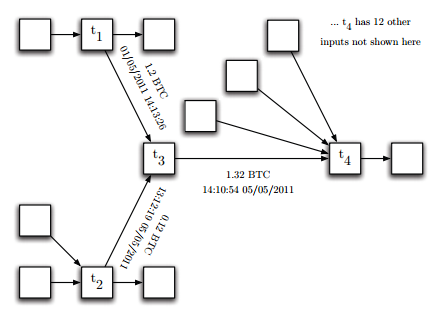
\includegraphics[height=6 cm]{images/anon_1.png}
			 \end{tabular}
		 \end{center}
 	\end{figure}

\end{frame}

\begin{frame}
	\frametitle{caso di studio: Reid [2011]}
	\framesubtitle{rete utenti imperfetta $\tilde{\mathcal{U}}$ }

	\begin{figure}[H]
	 	\begin{center}
			 \begin{tabular}{c @{\hspace{1em}} c}
				 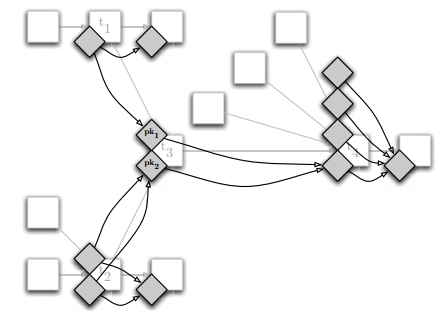
\includegraphics[height=6 cm]{images/anon_2.png}
			 \end{tabular}
		 \end{center}
 	\end{figure}
 
\end{frame}

\begin{frame}
	\frametitle{caso di studio: Reid [2011]}
	\framesubtitle{rete utenti $\mathcal{U}$, rete ancella $\mathcal{A}$}
	
	\begin{figure}[H]
	 	\begin{center}
			 \begin{tabular}{c @{\hspace{1em}} c}
				 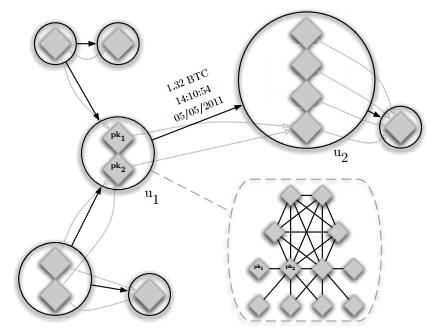
\includegraphics[height=6 cm]{images/anon_3.png}
			 \end{tabular}
		 \end{center}
 	\end{figure}

\end{frame}

\begin{frame}
	\frametitle{caso di studio: Reid [2011]}
	\framesubtitle{integrazione con informazioni esterne}
	
	\begin{itemize}
		\item dimensione $\propto |\{K_{PB}\}|$ utente = \# transazioni
		\item colore $\propto$ \bitcoinA \;scambiati
	\end{itemize} 
	
	\begin{figure}[H]
	 	\begin{center}
			 \begin{tabular}{c @{\hspace{1em}} c}
				 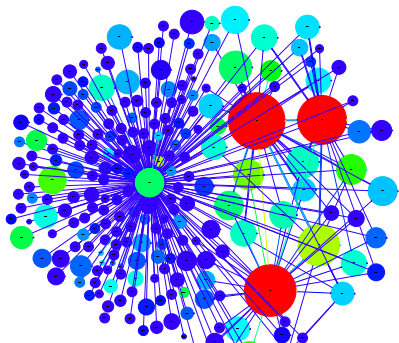
\includegraphics[height=6 cm]{images/anon_4.png}
			 \end{tabular}
		 \end{center}
 	\end{figure}

\end{frame}
\subsection{Double spending}
	%\begin{frame}
%	\frametitle{attacco semplice: Forking}
%	
%\end{frame}
% ----------------------------------------------------------------------------------------------------------------------------
\begin{frame}
	\frametitle{caso di studio: Karame [2012]}

	tipologia transazione 
	\begin{itemize}
	  \item \textit{lenta, e.g.} acquisto ticket eventi
	  		\newline $ \Rightarrow $ sicurezza offerta dal mining
	  \item \textit{{\color{blue}veloce}, e.g.} pagamento in negozio
	  		\newline $ \Rightarrow $ Karame: $\exists $ possibilità di double spending
	  		% negli attuali client, e ci sarebbero comunque se venissero seguite le sole
	  		% precauzioni suggerite prima di questo paper
	  		\begin{itemize}
	  			\item tempi scambio [s] $\ll$ tempi validazione [min]
	  			\item Bitcoin segue tecnica dello struzzo %SAY clients non tenuti ad attendere per transazioni DI POCO CONTO
	  			\item problema limitato in gravità ma non risolto
	  		\end{itemize} 
	\end{itemize}

\end{frame}
% ----------------------------------------------------------------------------------------------------------------------------
\begin{frame}
	\frametitle{caso di studio: Karame [2012]}
	\framesubtitle{garantire validità nel caso \textit{veloce}}

	% SAY curva di probabilità di risoluzione dei blocchi in un certo tempo.
	% 		modellizzata molto bene da una distribuzione geometrica spostata.
	%		quasi un terzo delle transazioni viene confermato in più di dieci minuti !

	\begin{figure}[H]
	 	\begin{center}
			 \begin{tabular}{c @{\hspace{1em}} c}
				 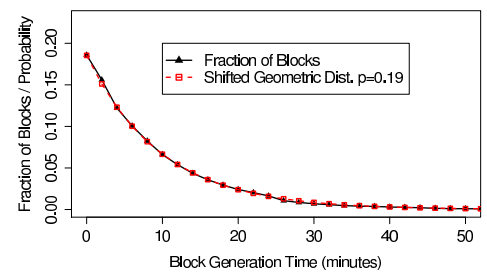
\includegraphics[height=5.5 cm]{images/dspending_1.png}
			 \end{tabular}
		 \end{center}
 	\end{figure}

\end{frame}
% ----------------------------------------------------------------------------------------------------------------------------
\begin{frame}
	\frametitle{caso di studio: Karame [2012]}
	\framesubtitle{ipotesi}

	% SAY curva di probabilità di risoluzione dei blocchi in un certo tempo.
	% 		modellizzata molto bene da una distribuzione geometrica spostata.
	%		quasi un terzo delle transazioni viene confermato in più di dieci minuti !

	\begin{columns}
	 \begin{column}{.45\textwidth}
		hosts
		\begin{itemize}
		  \item $A$ peer disonesto
		  \item $H$ complici di $A$ 
		  \item $V$ vendor onesto
		\end{itemize}
		transazioni
		\begin{itemize}
		  \item $\orange{\mathfrak{T}_V}$: acquisto regolare
		  \item $\orange{\mathfrak{T}_A}$: recupero fraudolento
		\end{itemize}
	\end{column}
	
	\begin{column}{.65\textwidth}
		ipotesi
		\begin{itemize}
		  \item $A$ conosce indirizzo IP di $V$
		  \item capacità di calcolo di $A$ trascurabile % %SAY a differenza della base comune agli attacchi di tipo lento
		  %SAY cioè diretta a indirizzi controllati da A
		  \item $\orange{\mathfrak{I}_V^{in}} = \orange{\mathfrak{I}_A^{in}} \in A$ 
		  \item $ V \ni\, \orange{\mathfrak{I}_V^{out}} \neq \orange{\mathfrak{I}_A^{out}} \in A$
		  \item implementazioni clients: \textit{plain vanilla} %SAY non utilizzate particolari contromisure
	 	\end{itemize}
 	\end{column}
 	\end{columns}

\end{frame}
% ----------------------------------------------------------------------------------------------------------------------------
\begin{frame}
	\frametitle{caso di studio: Karame [2012]}
	\framesubtitle{idea di massima}
 	
 	\begin{columns}
	 \begin{column}{.61\textwidth}
		\begin{itemize}	 
		  	\item $\orange{\mathfrak{T}_V}, \orange{\mathfrak{T}_A}$ inviate contemporaneamente
		  		\newline  $\;\;\Rightarrow $ incluse nello stesso pool %SAY ragionevole inclusione!
	  		\item se $\orange{\mathfrak{T}},\,\orange{\mathfrak{T^\prime}}$ condividono inputs 
	  			\newline $\;\;\Rightarrow $ non ammesse nello stesso pool
	  		\item inclusa solo la prima $\orange{\mathfrak{T}}$ ad arrivare
	  	\end{itemize}
	  	$\;\;\;\;\;\;\;\;\Rightarrow$
	  	\begin{itemize}
	  		\item $\orange{\mathfrak{T}_A}$ da validare rapidamente
	  		\item $\orange{\mathfrak{T}_V}$ sarà smentita dalla rete %SAY ma il vendor si affiderà ad essa intanto
		\end{itemize}
	 \end{column}
	
	 \begin{column}{.6\textwidth}
	 	\begin{figure}[H]
	 	\begin{center}
			 \begin{tabular}{c @{\hspace{1em}} c}
				 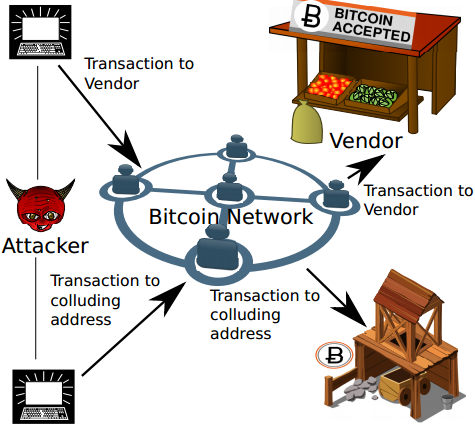
\includegraphics[height=5.5 cm]{images/dspending_2.png}
			 \end{tabular}
		 \end{center}
 		\end{figure}
	 \end{column}
	\end{columns}


% attack can succeed if V receives TRV ,and
% the majority of the peers in the network receive TRA so that TRA is more likely to be included in a subsequent block

\end{frame}
% ----------------------------------------------------------------------------------------------------------------------------
\begin{frame}
	\frametitle{caso di studio: Karame [2012]}
	\framesubtitle{$\mathbf{1^a}$ \textbf{condizione}: connessione diretta}
	
	\fbox{$V$\,riceve prima\,$\orange{\mathfrak{T}_V}$\,di\,$\orange{\mathfrak{T}_A}$}
		\, oppure\,$V$\,includerebbe prima\,$\orange{\mathfrak{T}_A}$\,nel pool
	
	\begin{columns}
		\begin{column}{.5\textwidth}
			\begin{itemize}
			  \item $A$ conosce IP di $V$
			  \item client accetta sempre nuove connessioni < 125 max
			  \item $A$ comunica con $H$
				\begin{itemize}
					\item senza latenza
					\item privatamente    
				\end{itemize}
			  \item $H$ non comunica con $V$
			  \item $A$ invia
				\begin{enumerate}
				  \item $\orange{\mathfrak{T}_V}$ a $V$
				  \item $\orange{\mathfrak{T}_A}$ a $H$
				\end{enumerate} %SAY il tempo a cui V riceve T_V è inferiore a quello in cui riceve T_A
			\end{itemize}
			 $\;\;\;\;\Rightarrow \orange{t_V^V} < \orange{t_V^A}$
		\end{column}
		
		\begin{column}{.60\textwidth}
			\begin{figure}[H]
		 	\begin{center}
				 \begin{tabular}{c @{\hspace{1em}} c}
					 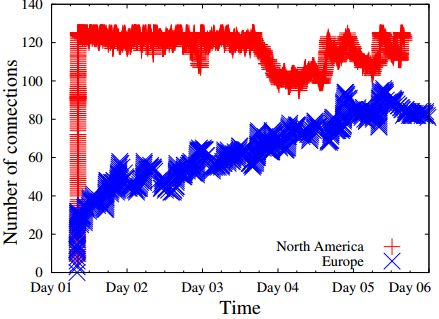
\includegraphics[height=4.75 cm]{images/dspending_3.png}
				 \end{tabular}
			 \end{center}
				\caption{analisi del momento propizio}
	 		\end{figure}
		\end{column}
	\end{columns}		  
\end{frame}
% ----------------------------------------------------------------------------------------------------------------------------
\begin{frame}
	\frametitle{caso di studio: Karame [2012]}
	\framesubtitle{$\mathbf{2^a}$ \textbf{condizione}: diffusione manipolata}
	
	\fbox{$\orange{\mathfrak{T}_A}$ inclusa in blockchain (\textit{i.e.} confermata) prima di
	$\orange{\mathfrak{T}_V}$} \vspace{0.1cm} \newline oppure $\orange{\mathfrak{T}_A}$ non potrebbe seguire $\orange{\mathfrak{T}_V}$ in blockchain
	  		
	\begin{itemize}
	  \item $H$,\,$V$ probabilmente lontani $\;\;\Rightarrow \orange{\mathfrak{T}_A}, \orange{\mathfrak{T}_V}$ broadcastate finchè 
  			$ \left \{
					  \begin{array}{lcr}
					    \text{ogni peer include}\;\orange{\mathfrak{T}_A}\:\dot{\vee}\:\orange{\mathfrak{T}_V}\;\text{in proprio pool}\\
					    \orange{\mathfrak{T}_A}\:\vee\:\orange{\mathfrak{T}_V}\;\text{è confermata}
					  \end{array}
					\right. $ 
	  \item $\Pr[\orange{\tau_A} < \orange{\tau_V}] \propto \sfrac{\orange{\eta_A}}{\orange{\eta_V}}$ governabile in due modi
	  		% TAU: tempo di inclusione in Blockchain
	  		% ETA: #peers che hanno incluso la transazione nel proprio pool
  		\begin{itemize}
  			\item invio di $\orange{\mathfrak{T}_A}$ precede invio di $\orange{\mathfrak{T}_V}$ 
  			\item $H$ aiutano $A$ diffondendo $\orange{\mathfrak{T}_A}$ e filtrando $\orange{\mathfrak{T}_V}$ 
  		\end{itemize}
	  \item ulteriori ipotesi
	  	\begin{itemize}
	  	  	\item $\exists$ istante ove $\orange{\mathfrak{T}_A},\,\orange{\mathfrak{T}_V}$ convivono
	  	  	\item $\forall\,\orange{\varepsilon}\;\mathrm{p.a.p.},\;\;\;
	  	  			\Pr[\orange{\tau_A}\sim\mathrm{secs}]\cup\Pr[\orange{\tau_V}\sim\mathrm{secs}]<\orange{\varepsilon}$ 
	  	  		%SAY HP: non è possibile che nessuna delle due sia confermata in pochi secondi dall'invio
  			\item $\orange{\eta_A},\,\orange{\eta_V}$ non scambiano blocchi risolti $\Rightarrow \orange{\tau_A},\,\orange{\tau_V}$ indipendenti
  			%the time required by peers that are mining in favor of TRV to generate a new block
  			%is independent of that required by the peers that are mining in favor of TRA 
	  	\end{itemize}
	\end{itemize}
	
	%probability of successful block generation in each δt can be modeled as a Bernoulli trial with success probability η p
	%	η is the number of peers  
	%	p the success probability of a peer in generating a block within δt

\end{frame}
% ----------------------------------------------------------------------------------------------------------------------------
\begin{frame}
	\frametitle{caso di studio: Karame [2012]}
	\framesubtitle{probabilità di successo}

	$\Pr[\text{successo in un tempo}\;\orange{\delta t}] \sim \mathrm{Bernoulli}(\orange{\eta},\,\orange{p})$
	\begin{itemize}
	  \item $\orange{\eta}=$ numero di peers coinvolti
	  \item $\orange{p}=\Pr[\,\text{peer generi un }\:\mathfrak{B}\:\text{in}\;{\delta t}\,]$ 
	\end{itemize}

	\begin{figure}[H]
	 	\begin{center}
			 \begin{tabular}{c @{\hspace{1em}} c}
				 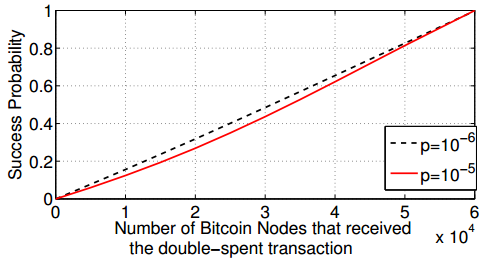
\includegraphics[height=4.5 cm]{images/dspending_4.png}
			 \end{tabular}
		 \end{center}
		 \caption{$\Pr[\mathrm{successo}\;|\;\delta t=10s,\;\eta=6\cdot10^4]$}
 	\end{figure}

 	%SAY dal numero di nodi che hanno ricevuto la doppia transazione, si può dare una stima della probabilità che qualche pool
 	% 	riesca a risolverla e a propagarla

\end{frame}
	%TODO eventualmente \begin{frame}
	\frametitle{Forking}

\end{frame}
	%GRINGO \begin{frame}
	\frametitle{Approfondimenti}
	\begin{itemize}
	  \item falsi miti \\
		\url{http://en.bitcoin.it/wiki/Myths}	  
	  \item frequently asked question \\
		\url{http://bitcoin.org/en/faq}	  
	  \item papers \\
	  	\url{http://en.bitcoin.it/wiki/Research}
	\end{itemize}
\end{frame}


% -------------------------------------------------------------------------
\end{document}